%!TEX root = jsba_main.tex
% This is the main file of my bachelorthesis


\documentclass[a4paper, 11pt]{article}

% Packages
\usepackage[utf8]{inputenc}
\usepackage[T1]{fontenc}
\usepackage{lmodern}
\usepackage[english]{babel}
\usepackage{moreverb}
\usepackage{textcomp}
\usepackage{url}
    % natbib
\usepackage[square,numbers]{natbib}
\usepackage[nottoc]{tocbibind}
\bibliographystyle{unsrtnat}
\setcitestyle{authoryear}
    % math
\usepackage{mathtools}
\usepackage{amsthm}
\theoremstyle{definition}
\newtheorem{exmp}{Example}[section]     % for examples
    % joins, etc.
\usepackage{amssymb}
\usepackage{ifsym}

    % todo
\usepackage{todonotes}

    % caption
\usepackage{caption}

% Distances, etc.
\setlength{\parindent}{0mm}
\setlength{\parskip}{1mm}


% Document
\begin{document}

% Title page & table of contents
%!TEX root = jsba_main.tex

%Titelseite
\newpage
\thispagestyle{empty}
\newcommand{\Rule}{\rule{\textwidth}{1mm}}

\begin{center}

\Rule\vspace{5mm}
\sffamily\bfseries\Huge
Similarity-based query answering for medical information systems
\vspace{1mm}\Rule
\vfill
\sffamily\bfseries\LARGE Bachelor Thesis
\vfill
\sffamily\bfseries\Large Jero Mario Schäfer\par Mat.nr.: 21552103\par Applied Informatics\par
\vfill

\raisebox{7mm}{Georg-August-University}
%\includegraphics[height=xxmm]{unilogo.pdf}
\raisebox{7mm}{Göttingen}\par
\vfill
\today
\end{center}


\newpage



\paragraph{Roter Faden für die Einleitung}

\begin{itemize}
    \item Distributed Database
    \begin{itemize}
        \item Was ist das?
        \item Vorteile, "Heute"
        \item ? Herausforderungen (-> in Bezug auf Anfragebeantwortung?)
        \item ? Apache Ignite?
    \end{itemize}
    
    \item Clustering-based Fragmentation
    \begin{itemize}
        \item Was ist das?
        \item ? Bezug zu MeSH? Im Beispiel mit MeSH?
        \item ? Ähnlichkeiten?
        \item ? medizinisches/klinisches Informationssystem?
        \item ? derived fragmentation
    \end{itemize}
    
    \item Flexible Query Answering (for SQL)
    \begin{itemize}
        \item Was ist das?
        \item Nutzen
        \item ? Beispiel? MeSH bzw. Informationssystem?
        \item ? Bezug zu DDBMS und Clustering-based fragmentation?\newline
                (\textrightarrow\,Inwiefern unterstützen o.g. Punkte das?)
    \end{itemize}
\end{itemize}



\paragraph{Theorieteil}

Alles etwas formaler? (Def. 1.: ..., Def. 2.: ... , Text ...)
Noch ein Schritt vor? Relationale Datenbanken, Relationales Datenmodell, ...

MeSH, UMLS ?

\begin{itemize}
    \item DDBs
    \begin{itemize}
        \item Begriffserklärungen/-definitionen\textrightarrow Glossar??? Abkürzungsverzeichnis???
        \item Architektur (Client-Server, Data/Computing Nodes, homogen/heterogen)
        \item Konzepte, Replikation und Fragmentierung (Datenverteilung)
        \item Distributed SQL, Query processing/optimization???
    \end{itemize}
    
    \item ...
\end{itemize}




% TODO-List
\listoftodos
\newpage
\tableofcontents

% Introduction
\newpage
%!TEX root = jsba_main.tex
% Introduction

\section{Introduction}
\label{sec:intro}

\emph{Distributed databases} (DDBs) gained significantly more importance over the past years as they provide physically distributed storage \citep{Tan2009}
for the ever-growing amount of data in our world. Especially, in fields where the amount of data to be hosted in a database is challenging, e.g. multimedia
and textual data occurring in a social network with millions of people or medical so-called "big data" retrieved and collected from different sources to be
used in healthcare for e.g. predictions or research as mentioned in \citet{Lee2017}, a fragmentation and replication of this big data to multiple servers 
in a cloud storage infrastructure instead of one single server can pay off. The data fragmentation overcomes the limitation of storage capacity of a single
storage instance as the total amount of data can be split into smaller parts, so-called fragments, and fragmentation can increase the performance of the 
query processing. 
Furthermore, the replication of the data fragments inside the network yields a tolerance to failures by compensating data loss with recovery, e.g. in 
case of a malfunction or total failure of a single server, to guarantee the desired availability and reliability of the data accessed by the users of the
distributed database system (DDBS).


In the case of a relational data model underlying the database, a fragmentation of the data can be a \emph{horizontal} or \emph{vertical fragmentation} 
of the relations (tables) of the database \citep[pp.~104f.]{Ozsu1991}. A horizontal fragmentation means a tuple-wise assignment to fragments, i.e. fragments
contain subsets of rows of the non-fragmented table, whereas a vertical fragmentation "slices" the relation by its attributes, i.e. fragments contain
projections to the columns. 
The here analyzed and implemented approach uses a clustering heuristic on one chosen attribute as described in \citet{Wiese2014} to obtain a primary
horizontal fragmentation for a relation. The clustering procedure depends on a similarity calculation of the values of the chosen relaxation attribute 
resulting in a clustering of the column's values, such that values with a high similarity belong to the same cluster. Hence, a fragmentation of relations
that have common attributes with this horizontally fragmented relation, i.e. attributes that will be used in queries to join these two relations, can be 
\emph{derived}~\citep[pp.~116f.]{Ozsu1991}, such that the tuples which are about to be joined reside on the same server allowing for better performance in 
queries compared to query processing with a distributed join which has to be applied if the data is not residing at the same
site~\citep{Sattler2009DistJoin}.
Thus, this derived horizontal fragmentation improves data locality~\citep{Wiese2014} because the probably high delay of data transmission over the 
network, which is needed in case of a distributed join, will be avoided to the joy of any database user.


\defcitealias{MeSH}{MeSH\textcopyright}
The example of a \emph{medical information system}, which is used as an application of such a distributed database system with a clustering-based 
fragmentation, is a modified version of the example defined in \citet{Wiese2014}. Patient's personal information as well as the diseases they suffer from
are contained in a distributed database. For example, a hospital could host this database to provide access to the patient data to doctors and nurses that
need to work with this data from different computers or other technical devices located in the hospital, but it is also possible that researchers could
make use of that patient data, e.g. when investigating the co-occurrence of several diseases.
The clustering procedure is applied to this disease information of patients, whereas the disease terms are conform to the vocabulary provided by the 
\emph{Medical Subject Headings} taxonomy (see \citetalias{MeSH}) of the U.S. National Library of Medicine, which is the largest biomedical library in 
the world. The \emph{Unified Medical Language System} (UMLS), which was also developed and maintained by the U.S. National Library of Medicine, brings
together several taxonomies, like the MeSH taxonomy, in order to integrate and link their biomedical and health-related vocabularies allowing applications
to interchange information based on different vocabularies.
A similarity measure defined between the disease terms from the MeSH database yields the needed similarity calculation for the clustering-based 
fragmentation. In this way, tuples holding information about patients suffering from similar illnesses are stored on the same site and can easily be
queried together in an intelligent, non-distributed fashion.


Upon query failure, i.e. when the database cannot give an exact answer to a query formulated by a user, an empty result is returned. Assuming the query 
was formulated correctly, the blank result indicates to the user that the information he or she was looking for is not present in the current database
state due to the lack of any exact answers, and so this result is non-informative for the user in the general case. \emph{Flexible query answering}, on 
the contrary, can overcome this lack of information when the database system uses techniques like \emph{query generalization} to provide the user a 
non-empty result, which on the one hand does not match the query exactly but on the other hand contains information instead that may be relevant to the
user.

\begin{exmp}
\label{sec:intro_exmp}
Consider a sample database about companies and their employees. The database contains a relation 'Employee' with information about a person, e.g. the
person's name, age, address, salary, social security number and a reference to the company the person works for. The companies are stored in the
relation 'Company' that has the attributes name, headquarter, industrial sector and maybe some others. An exemplary SQL query that joins the two relations
to find out the name of those companies in a certain business where the average salary of all employees is higher than 100.000~\$ could be
\begin{verbatim}
    SELECT Company.name 
    FROM Employee, Company 
    WHERE Employee.Company = Company.Name 
        AND Company.Industry = 'Farming'
    GROUP BY Company.Name 
    HAVING avg(salary) > 100000.
\end{verbatim}
However, as the database maybe does not know a company from that agricultural sub-sector having an average salary like that, it could return an empty 
answer to the query that is not satisfying for the user. Instead of returning and empty answer set, the database could - of course only if it is able 
to do so - try to answer the given query in a flexible manner, e.g. by changing the selection condition in the \verb!WHERE! clause
\begin{verbatim}
    Company.Industry = 'Farming'
\end{verbatim}
to a more \emph{general} one that could provide some information not matching the query exactly but still having some informational content. One way to 
achieve this, would be to omit this selection condition completely from the \verb!WHERE! clause resulting in a possibly non-empty answer that would 
contain names of companies from all industrial sectors that suffice the stated average salary condition. A more relevant answer for the user could be
obtained by first generalizing the sub-sector farming to the broader sector of agriculture that includes for example fishing companies as well as the
forestry sector. Thereby, not all industrial sectors, which include companies that might have nothing in common with the intended agricultural companies,
are considered but only those that are of the user's interest. The higher relevance of the informational content from an answer of the database to an in 
this way rewritten query compared to the first approach is achieved by allowing \emph{similar} answers in case of query failure.
\end{exmp}

As shown previously in Example~\ref{sec:intro_exmp}, the \emph{similarity-based, flexible query answering} \citep{Wiese2014} enables the database in case 
of a failing query, which is possibly not satisfying for the user, to search for answers in closely related sectors regarding the chosen attribute, 
the \emph{relaxation attribute} \citep{Wiese2014}, by taking those values of the domain of the relaxation attribute into account that actually have some 
relatedness to the initally stated query which suffices to satisfy the user's needs. In contrast to this, an extension of the query sent to the
database without any modified selection condition on the relaxation attribute might have answers that have not necessarily any relatedness to the initial
query, thus, they are not really informative for the user unless he filters out those tuples matching his question most.


\defcitealias{UMLS::Sim}{UMLS::Similarity}
The "HIGHmed" project \citep{Haarbrandt2018} is an approach to develop an open infrastructure for information exchange and data management and integration
in order to facilitate and improve research and health care as a cooperation of three German university hospitals and the German Cancer Research Center
(DKFZ) as the core partners together with other partners, e.g. from research institutions or from the industry (cf. \cite[Table~2]{Haarbrandt2018}.
Indeed, the similarity plays a big role today in the health care section as indicated in the oncology use case in the article to the project.
For this, the developed platform will incorporate a "virtual oncology center" (VOC) \citep{Haarbrandt2018} with the goal to improve clinical research and 
decision making regarding cancer diseases by a functional infrastructure. This part of the platform aims to utilize shared data about courses of
treatment of patients and historical data from studies, which are provided from different participating sources, with applications built on this platform.
By doing so, the applications support the identification of similar cases for selected patients in order to help to decide for an appropriatly tailored
treatment and to be able to draw conclusions regarding the disease progression. The used similarity measures that enable the search for similar patients,
whose pathologies and treatments lead to inference of useful knowledge for the decision making, depend on machine learning and ontologies. The latter ones
also form the core part for the tool of the \citetalias{UMLS::Sim} module, developed by \cite{McInnes2009}, which will be used later in the underlying
implementation of the distributed database system to calculate similarities between disease terms according to the Medical Subject Headings taxonomy 
(see \citetalias{MeSH}) that are required for the clustering-based fragmentation as well as the similarity-based query answering.


In the following section there will be given a theoretical introduction about distributed database systems in general with the underlying distribution 
concepts of data replication and fragmentation and about the distributed query processing that plays a big role in a distributed database. 
Section~\ref{sec:meth} describes the methods that are used to implement a medical information system that is built with the help of an in-memory database
system and distributes the data according to a clustering-based fragmentation which enables for similarity-based and flexible query answering.
Section~\ref{sec:impl} encompasses the technical details and conditions of the implementation of the system, namely two alternative implementations and
a reference implementation, the clustering procedure and (flexible) query answering and rewriting. Based on this implementation, Section~\ref{sec:res}
illustrates and evaluates the results of query executions with the system in the different implementation alternatives.

\todo[inline]{Summarize content of the missing sections \dots}

% Theoretical Background: Distributed Databases, ...
\newpage
%!TEX root = jsba_main.tex
% Theoretical background 

\section{Theoretical Background}
\label{sec:theo}

In the following section there first will be given an introduction to the distributed database terminology and the further subsections give an overview of
the architecture, fragmentation and replication that take place in such distributed systems as well as some advantages and disadvantages. The second 
section outlines the distributed query processing, which is required when querying for physically distributed data, and gives some insights in how queries
can be decomposed and rewritten to match the distribution of the data in an optimized way.

\subsection{Distributed Databases}
\label{sec:theo_ddb}

\subsubsection{Terminology}
\label{sec:theo_ddb_term}
A \emph{distributed database}~(DDB) can be defined as multiple, logically interconnected databases spread across a computer network~\cite[p.~4]{Ozsu1991},
such that the physical presence of the data may be dispersed spatially instead of having one single database hoarding all the data at a certain location
physically. On top of this DDB, there is often a so-called \emph{distributed database management system}~(DDBMS) which manages the underlying databases 
and the access to the data, and the users are enabled to work with the data of the DDB without noticing the physically distribution, i.e. in a transparent 
manner~\cite[pp.~4f.]{Ozsu1991}.
This results, from the point of view of a user, in a logically single database, which can be queried in the same way as a non-distributed database. 
Furthermore, users can benefit from a physical distribution of the data depending on an architectural design because they can communicate with the 
geographically closest site where one of the databases resides reducing the network communication delay, and concurrent access of the DDB can be handled 
in a distributed way, too, exploiting the fact that more servers imply more computing power for the \emph{distributed database system}~(DDBS).
Additionally, a DDBS can provide an improved availability compared to a non-distributed database, e.g. when the data is replicated. This implies that the
data can be reached from multiple sites even if there is a failure of one of the databases or of parts of the communication network. In this way, users
will have a chance to be able to still retrieve the data regardless of parts of the database being not available.


\subsubsection{Architecture}
\label{sec:theo_ddb_arch}
\defcitealias{Ignite}{Apache Ignite\texttrademark{}}
An architecture of a distributed database mangement system could look like depicted in Figure~\ref{fig:ddbs_arch}. Four different locations interconnected
via a communication network are each holding a database which is connected to a DBMS managing the underlying database. The locations can be local, e.g.
four computers or servers in one room, or global, e.g. four servers at different cities where the company holding this DDBS resides. The type of a DDBMS
can be classified as \emph{homogenous} or \emph{heterogenous} where in a homogenous DDBS all participating sites share the same DBMS locally and in a
heterogenous DDBS the sites may have a different DBMS with probably different data models \cite[p.~607]{Ramakrish2000}. For example, if in
Figure~\ref{fig:ddbs_arch} all DBMSs (DBMS 1 -- DBMS 4) are the same DBMS, e.g. all are \citetalias{Ignite} nodes, then the distributed database system
would be homogenous (cf. \cite[Fig.~2]{Jadhav2017}). If at least one of the locations is in control of a second DBMS, the DDBS would be homogenous, which
is also called a \emph{multidatabase system}. However, the heterogenity of a DDBS introduces "a significant cost in terms of performance, software
complexity, and administration difficulty" \cite[p.~608, l.13--14]{Ramakrish2000} regarding the management of the distributed data.

\begin{figure}[h]
    \centering
    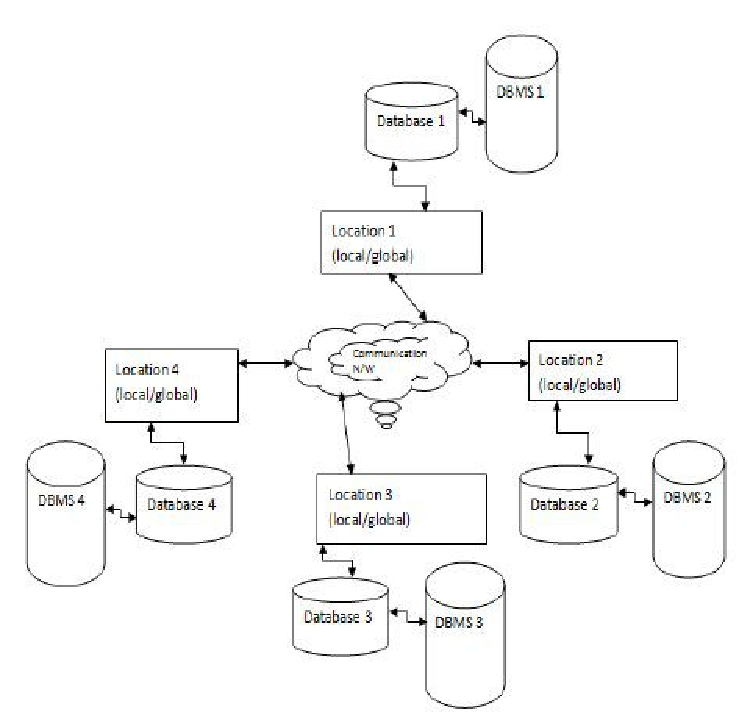
\includegraphics[width=0.8\textwidth,keepaspectratio=true]{img/DDBMS_Architecture.pdf}
    \caption{Architecture of a distributed database system from \cite[Fig.~1]{Kumar2013}}
    \label{fig:ddbs_arch}
\end{figure}

In \citet[pp.~608f.]{Ramakrish2000} the three architecture approaches, \emph{Client-Server}, \emph{Collaborating Server} and \emph{Middleware}, are 
discussed. The first, really popular architectural model is characterized by a distinction between client and server processes resulting in a separation of
functionality, i.e. servers are responsible for data storage and management whereas clients provide user interfaces to query data from a server. In a
Collaborating Server system, in contrast, all servers are able to decompose received queries that concern data from multiple servers to subqueries. The
subqueries are then executed accordingly at the servers on their locally stored data and a result is computed from all the servers' answers. This is also
described in Section~\ref{sec:theo_dqp}. In Middleware systems the task of query management and decomposition is handled by a single server and all other
servers only need to perform queries against their local data.



\subsubsection{Fragmentation}
\label{sec:theo_ddb_frag}
The relations of distributed databases can be partitioned into fragments of the relations, i.e. the data from the tables is split up and assigned to one 
or more of the databases that belong to the DDBS. The amount of data per database can be reduced by doing so. This \emph{fragmentation} can be achieved 
by using a certain fragmentation strategy and the resulting fragments, which contain parts of the whole data set, can then be dispersed across the network
by mapping the fragments to databases that possibly reside at different physical locations which are not necessarily geographically distant. The in the
following introduced fragmentation alternatives will be elucidated by ways of small "toy" examples in Example~\ref{sec:theo_ddb_exmp}.

One strategy to obtain a fragmentation of the data is the so-called \emph{horizontal fragmentation} \cite[p.~105]{Ozsu1991} that divides a relation in a 
row-wise manner into smaller portions with only some of tuples that were contained in the original relation, i.e. a relation $R$ can be divided into 
fragments $F_1, F_2,\dots, F_n$ by assigning each tuple $\mu$ of the relation $R$ to at least one fragment $F_i,~i\in\{1,\dots,n\}$. The result of this is
that for all $i\in\{1,\dots,n\},~F_i \subseteq R$. Additionally, if there is no replication (cf. Section~\ref{sec:theo_ddb_repl}) applied to the data and
each tuple is only assigned to exactly one fragment, the fragments are pairwise disjoint ($\forall \mu \in F_i$ it holds that 
$\mu \notin F_j, i\neq j, i,j\in\{1,\dots,n\}$) if the relation $R$ does not contain any duplicate tuples itself. In the relational algebra such a
\emph{primary horizontal fragmentation} can be described by a selection operation on the relation $R$ \cite[p.~109]{Ozsu1991}, whereas the selection 
condition defines the wanted mapping of tuples to fragments. Regarding this primary horizontal fragmentation, a further fragmentation of another relation
$S$ can be \emph{derived} by computing the semi-join of the relation $S$ with fragments $F_i,~i\in\{1,\dots,n\}$ of the primary relation $R$
\cite[pp.~116f.]{Ozsu1991}, i.e. the derived fragments $G_i$ of the relation $S$ are computed as $G_i=S \ltimes F_i$ for $i\in\{1,\dots,n\}$.
The \emph{derived horizontal fragmentation} depends on the underlying primary horizontal fragmentation, and, to prevent tuples in $S$ from getting lost
during the semi-join with fragments of $R$, it is necessary to have for each tuple $y\in S$ matching tuples in $R$ in order to let the tuples from $S$ 
"survive" the semi-join. An integrity constraint in form of a foreign key reference of the relation $S$ to the relation $R$ can be used to enforce this
condition for the sake of completeness of the derived fragmentation. Inherently with the definition of the derived horizontal fragmentation on a semi-join,
replication of tuples of $S$ in the derived fragments may occur if tuples in $S$ match multiple tuples that belong to different fragments of 
$R$ \cite[p.~121]{Ozsu1991}. This causes the fragments $G_i$ of $S$ not to be disjoint in general which is equal to a partial replication as described 
in Section~\ref{sec:theo_ddb_repl}.


On the other hand, a \emph{vertical fragmentation} \cite[p.~122]{Ozsu1991} is a columnwise division of a relation $R$, such that each of the resulting
fragments $F_1,F_2,\dots,F_n$ has a subset of the attributes of the relation $R$. To identify the original tuple to which a partitioned tuple of one of 
the fragments belongs to, it is necessary to have a primary key defined on the relation $R$ which can be stored with the subset of attributes of the 
tuple that is assigned to a fragment. If it is not the case that a primary key is set for the relation $R$, then an abstract, maybe randomly generated
unique identifier has to be introduced, i.e. as additional attribute, in order to match tuple fragments to their source. 

Another fragmentation strategy, which will only be mentioned here and not further analyzed, is the so-called \emph{hybrid fragmentation} or 
\emph{nested fragmentation} \cite[pp.~135f.]{Ozsu1991} that can be achieved by nesting horizontal and vertical fragmentations on a relation giving a 
complex partitioning of the data and arising lots of issues to consider when implementing an application based on data that is fragmented by such type 
of fragmentation strategy.

\begin{exmp} \label{sec:theo_ddb_exmp}
$ $\newline
    \begin{center}
    \begin{tabular}{|c|c|} 
        \hline
        $a$ & $b$ \\
        \hline
        0 & x \\
        1 & x \\
        2 & y \\
        3 & z \\
        7 & g \\
        \hline
    \end{tabular}
    \captionof{table}{Relation $R$ with primary key $a$ and attribute $b$ (foreign key on $S.b$; see Table~\ref{tab:s})}
    \label{tab:r}
    \end{center}
$ $\newline
Consider having three fragments $F_1$, $F_2$ and $F_3$ of the relation $R$ which contains the tuples $\{(0,x), (1,x), (2,y), (3,z), (7,g)\}$ over the 
attributes $a$ and $b$, as shown in Table~\ref{tab:r}. 
A possible horizontal fragmentation is $F_1=\{(0,x), (1,x)\}$, $F_2=\{(2,y), (3,z)\}$ and $F_3=\{(7,g)\}$. 
This fragmentation is illustrated by Table~\ref{tab:r_frag} and could be obtained from the three selections $F_1=\sigma_{a \leq 1}(R)$,
$F_2=\sigma_{a \geq 2~\land~a \leq 5}(R)$ and $F_3=\sigma_{a \geq 6}(R)$. Here, each row of the table, i.e. each tuple $\mu \in R$, is assigned to 
exactly one of the fragments $F_i,~i\in\{1,2,3\}$, so there is no duplication of any tuple and the fragments are pairwise disjoint, but each tuple 
$\mu \in R$ is somewhere contained in one of the fragments. Hence, the union $F_1 \cup F_2 \cup F_3$ of all the fragments yields the original tuple set,
which means that the partitioned relation $R$ can be reconstructed from the fragments, because each of the original tuples is found in (at least) one
fragment. Due to the fact that this primary horizontal fragmentation is complete and disjoint and that the fragmentation can be reverted by reconstruction
of the original relation, the three fragmentation correctness rules \cite[p.~103]{Ozsu1991} are fulfilled.

\begin{table}[h]
    \hspace*{\fill}
    \begin{tabular}{|c|c|}
        \hline
        $a$ & $b$\\
        \hline
        0 & x \\
        1 & x \\
        \hline
    \end{tabular}
    \hfill
    \begin{tabular}{|c|c|}
        \hline
        $a$ & $b$\\
        \hline
        2 & y \\
        3 & z \\
        \hline
    \end{tabular}
    \hfill
    \begin{tabular}{|c|c|}
        \hline
        $a$ & $b$\\
        \hline
        7 & g \\
        \hline
    \end{tabular}
    \hspace*{\fill}
    \caption{Horizontal fragments $F_1$, $F_2$ and $F_3$ (from left to right)}
    \label{tab:r_frag}
\end{table}

According to this primary horizontal fragmentation of $R$, a derived horizontal fragmentation of $S=\{(x, 0.5), (y, 0.3), (g, 9.9)\}$ (Table~\ref{tab:s})
over the attributes $b$ and $c$ is obtained by computing the previously stated definition using a semi-join, fragment $G_i = S \ltimes F_i$ for
$i\in\{1,2,3\}$. Based on the matches of tuples from $S$ with tuples in the fragments $F_i$, the derived fragments are 
$G_1=\{(x,0.5)\}$, $G_2=\{(y, 0.3)\}$ and $G_3=\{(g, 9.9)\}$ (Table~\ref{tab:s}).


\begin{table}[h]
    \hspace*{\fill}
    \begin{center}
    \begin{tabular}{|c|c|}
        \hline
        $b$ & $c$\\
        \hline
        x & 0.5 \\
        y & 0.3 \\
        g & 9.9 \\
        \hline
    \end{tabular}
    \hspace{20pt}
    \begin{tabular}{|c|c|}
        \hline
        $b$ & $c$\\
        \hline
        x & 0.5 \\
        \hline
    \end{tabular}
    \hspace{5pt}
    \begin{tabular}{|c|c|}
        \hline
        $b$ & $c$\\
        \hline
        y & 0.3 \\
        \hline
    \end{tabular}
    \hspace{5pt}
    \begin{tabular}{|c|c|}
        \hline
        $b$ & $c$ \\
        \hline
        g & 9.9 \\
        \hline
    \end{tabular}
    \caption{Relation $S$ with attributes $b$ and $c$ (leftmost), derived fragments $G_1$, $G_2$ and $G_3$}
    \label{tab:s}
    \end{center}
\end{table}

For the demonstration of an exemplary vertical fragmentation, consider the view $T$ calculated as the left outer join of the two relations $R$ and $S$, 
$T~=~R~{\tiny \textifsym{d|><|}}~S$ over the attribute set $\{a,b,c\}$. 
This left outer join yields the tuple set (see Table~\ref{tab:join_vert_frag})
\[
\{(0,x,0.5), (1,x,0.5), (2,y,0.3), (3,z,null), (7,g,9.9))\}.
\]
The so obtained relation (or view) can be partitioned vertically based on the two attribute subsets $\{a,b\}$ and $\{b,c\}$ that produce two vertical
fragments $H_1$ and $H_2$, which are also depicted in Table~\ref{tab:join_vert_frag} next to the original relation. Here, each tuple of one of the 
vertical fragments contains the attribute a, which is, in this case, a unique identifier for the original tuple from $T$.

\begin{table}[h]
    \centering
    \begin{tabular}{|c|c|c|}
        \hline
        $a$ & $b$ & $c$ \\
        \hline
        0 & x & 0.5 \\
        1 & x & 0.5 \\
        2 & y & 0.3 \\
        3 & z & null \\
        7 & g & 9.9 \\
        \hline
    \end{tabular}
    \hspace{30pt}
    \begin{tabular}{|c|c|}
        \hline
        $a$ & $b$ \\
        \hline
        0 & x \\
        1 & x \\
        2 & y \\
        3 & z \\
        7 & g \\
        \hline
    \end{tabular}
    \hspace{10pt}
    \begin{tabular}{|c|c|}
        \hline
        $a$ & $c$ \\
        \hline
        0 & 0.5 \\
        1 & 0.5 \\
        2 & 0.3 \\
        3 & null \\
        7 & 9.9 \\
        \hline
    \end{tabular}
    \caption{$R~{\tiny \textifsym{d|><|}}~S$, vertical fragments $H_1$ and $H_2$}
    \label{tab:join_vert_frag}
\end{table}

\end{exmp}



\subsubsection{Replication}
\label{sec:theo_ddb_repl}
The \emph{data replication} as discussed in \citet{Wiese2014} is not relevant for the implementation part in this work, and so this topic will only be
mentioned here and the investigations on it will be kept short as it still is an important part of distributed databases. Replication is a design approach
for a DDBS that is used for storing the data together with copies of the data. The data is duplicated and can be distributed multiple times to even 
different sites such that a the same data is present on different servers. In contrast to this, the data can also be \emph{partitioned} where none of the
data fragments, which are obtained from a fragmentation as analyzed in Section~\ref{sec:theo_ddb_frag}, is duplicated. There exist two alternative basic
strategies for a replication design \cite[p.~12]{Ozsu1991}. One of them is the \emph{full replication} where the whole database is stored at each site,
i.e. the data is distributed to each server and so each server has exactly the same data set as all other servers. The other one is the 
\emph{partial replication} where each of the data partitions can distributed to more than one server. A partial replication for example could be used in
case of having each partition at a server that is primarily responsible for that partition (primary partition) and at some other servers where the
partitions are held as backup copies for the primary partition.


\subsubsection{Advantages and Disadvantages of DDBMS}
Using distributed databases for storing and managing information can be advantageous. As already mentioned, the distribution of the data across multiple 
servers can provide features like higher availability of the data, which can come from failure tolerance, as well as more efficient interaction with the
DDBS. Several advantages of distributed database systems are (cf. \citep{Jadhav2017} and \cite[pp.~8ff.]{Ozsu1991}):

\begin{enumerate}
    \item Local Autonomy: Data that is frequently accessed from a certain user group can be placed at the site which is the closest one to the user group
            allowing for local control and indepent access.
    \item Improved Performance: Parallelizing queries and resource usage can lead to higher efficiency.
    \item Improved Reliability/Availability: Distributed data has a higher resistance to inaccessibility in case of a failure because it may be retrieved 
            from another site and work on at least the part of the data which is not affected by a failure can be guaranteed. 
    \item Expandability: The DDBS can be simply expanded by e.g. additional servers that improve the load balancing abilities of the system
    \item Shareability: Distributed databases inherently offer the possibility to share the stored data
\end{enumerate}

On the contrary, one big disadvantage of a DDBS is that installation, control and maintenance of such a system are really hard because of the way
more complex appearance of a DDBS compared to the centralized database concept \citep{Jadhav2017}. The design of a DDBS is also crucial as it can cause 
the system to be less efficient if the design is not well-suited to the application's requirements what can lead to bad resource usage and high
communication costs in the interconnecting network. More issues are security of system and data, which demand some extra effort in terms of protection
because the sites and data fragments are not centralized but remote making them more vulnerable if not secured accordingly, and economics where more
infrastructure and hardware for a distribution to multiple sites come along with higher costs \cite{Kumar2013}.


\subsection{Distributed Query Processing}
\label{sec:theo_dqp}
As the data is physically distributed, queries have to be processed and rewritten according to the underlying distribution to allow for an appropriate
answer to the given question. This section gives a brief insight in the mechanisms of processing distributed queries by applying transformations, rewriting
rules and optimization strategies.

\subsubsection{Overview}
\label{sec:theo_dqp_over}
A relational DDBS has to be able to answer a query in the same manner as a non-distributed relational database. The result of a query is a set of tuples
fulfilling the query. To obtain such a set the database system uses relational algebra operations for its computation, e.g. a join of two tables or the
selection on an attribute with a certain condition. When now considering distributed data, which could be fragmented and replicated, the performance of
computing answers to the query can be a big issue due to increased network communication inferred by data transfer between the database sites 
\cite[p.~173]{Ozsu1991}. This can even occur for simple queries that only scan a certain relation and project to some subset of the attributes.


\begin{exmp} \label{sec:theo_dqp_exmp}
Again, examine a similar situation as in Example~\ref{sec:theo_ddb_exmp} regarding the data from Table~\ref{tab:r} and Table~\ref{tab:s}. For example, 
assume that both relations $R$ and $S$ are neither fragmented nor replicated but distributed in such a way that one server holds all the tuples of 
relation $R$ and another server holds all the tuples of relation $S$ as shown in Figure~\ref{fig:dqp_rs_simple}.


\begin{figure}[h]
    \centering
    \framebox[0.8\textwidth]{
        Servers
        \hspace*{1cm}
        \framebox[1.2\width]{
            $S_1$
            \hspace{0.5cm}
            \begin{tabular}{|c|c|} 
                \hline
                $a$ & $b$\\
                \hline
                0 & x \\
                1 & x \\
                2 & y \\
                3 & z \\
                7 & g \\
                \hline
            \end{tabular}
        }
        
        \hspace*{1cm}
        
        \framebox[1.2\width]{
            $S_2$
            \hspace{0.5cm}
            \begin{tabular}{|c|c|}
                \hline
                $b$ & $c$\\
                \hline
                x & 0.5 \\
                y & 0.3 \\
                g & 9.9 \\
                \hline
            \end{tabular}
        }
    }
\caption{Distribution of relations $R$ (Table~\ref{tab:r}) and $S$ (Table~\ref{tab:s}) to two servers $S_1$ and $S_2$}
\label{fig:dqp_rs_simple}
\end{figure}


Then, a rather simple query without any joins and only one relation concerned like
\begin{verbatim}
    SELECT R.a FROM R WHERE R.b = 'x'
\end{verbatim}
can be evaluated - in this case easily - by the DDBMS by sending the query only to server $S_1$ in order to correctly fetch the tuples for the result from
there. The knowledge about the distribution of relation $R$ and $S$ enables the DDBMS to decompose and optimize the query. But upon a join, querying is not
that simple anymore due to the fact that now tuples have to be fetched from multiple servers and be combined with one another. 
For example, have a look at the query
\begin{verbatim}
    SELECT R.a, R.b, S.c FROM R, S WHERE R.b = S.b AND S.c < 1
\end{verbatim}
which could be answered, e.g. by sending all the tuples in $S$ from $S_2$ to $S_1$ which would then be joined and selected locally and the result would be
returned. Instead of sending all tuples in $S$ from $S_2$ to $S_1$, the selection condition \verb!S.c < 1! could be pushed down and evaluated locally on 
$S_2$ to improve the execution by reducing the amount of tuples that has to be sent via the network. This results in a decrease of the by data transfer
implied delay. Another possibly even more efficient computation could be done by decomposing the query and sending the subquery
\begin{verbatim}
    SELECT S.b FROM S WHERE S.c < 1
\end{verbatim}
to the server $S_2$ and the subquery
\begin{verbatim}
    SELECT * FROM R
\end{verbatim}
to the server $S_1$. The results of both queries could then be joined locally at the client-side 
(cf. Client-Server architecture from Section~\ref{sec:theo_ddb_arch}) or at a third server which is responsible for the query processing 
(cf. Middleware architecture from Section~\ref{sec:theo_ddb_arch}).

\end{exmp}

The Example~\ref{sec:theo_dqp_exmp} indicates the requirement and the possibilities of \emph{distributed query processing} strategies that allow for
transforming a query stated against the database, e.g. written in SQL, into an execution plan consisting of relational algebra instructions for the
database which yield the correct result set for the query in an optimal way (cf. \cite[p.~174]{Ozsu1991}, \citep{Sattler2009DistQuer}). However, under a 
distributed environment, the relational algebra alone is not sufficient to process the queries as it lacks operators for sending and retrieving data from
another server to complete the answer computation \cite[p.~175]{Ozsu1991}, thus, distributed query processing strategies come along with more difficulties.
Because of this and because of the widespread subproblems, that range from the used languages over the optimized resource usage to the possibilities and 
issues brought into the system by fragmentation and replication, only several chosen aspects will be discussed in the following.


\subsubsection{Query Decomposition \& Data Localization}
\label{sec:theo_dqp_decomp}

\emph{Query decomposition} means the process of rewriting the query to a normalized form (cf. \cite[p.~21,pp.189f.]{Ozsu1991}), followed by a semantical
analysis, a simplification of the query and a rewriting and restructuring to a relational algebra query \cite[p.~183]{Ozsu1991}. These four steps provide
as their result an algebraic query that can be optimized, e.g. as discussed in Example~\ref{sec:theo_dqp_exmp} for a SQL query where sending all tuples
from one server to another server is obviously less efficient than reducing the amount of data that has to be transmitted across the network between the
servers, whereas the real optimization is applied to the rewritten algebraic query, which can be displayed by a \emph{relational algebra tree}
(cf. \cite[Figure~8.3, p.~195]{Ozsu1991}), and not to the SQL query directly. The actual distribution of the data does not play any role here because
yet only global relations are considered when transforming into an algebra query.

Fragmentation and replication, as discussed in Section~\ref{sec:theo_ddb_frag} and Section~\ref{sec:theo_ddb_repl}, respectively, influence the query
execution strategy as they require for a distribution of the query itself to possibly multiple servers, too, in order to get the complete and correct 
result set. For the sake of simplicity and due to the fact that the replication will not be implemented later, it is assumed that the data is only 
fragmented horizontally and not replicated, i.e. every tuple is assigned to exactly one fragment. This also enables for the reconstruction of the original,
global relations by reverting the fragmentation. This so-called \emph{localization program} \cite[p.~199]{Ozsu1991} obtained by reverting the 
fragmentation can be expressed as operations of the relational algebra. This was already discussed in Example~\ref{sec:theo_ddb_exmp} where the
fragmentation of the relation $R$ was reversible by the union of all the horizontal fragments of $R$. Hence, a very simple, but rather inefficient way to
rewrite the actual pyhsical distribution of the data into the query is to substitute each global relation in the algebra query by its localization program 
\cite[p.~199]{Ozsu1991}.

\begin{exmp}
\label{sec:theo_dqp_exmp2}
Consider again the relation $R$ and its horizontal fragmentation as introduced in Example~\ref{sec:theo_ddb_exmp} and the query on the global relation $R$,
\verb!SELECT R.a FROM R!. The according localization program is $R=F_1 \cup F_2 \cup F_3$, and this query would have to be rewritten as - for better
readability in SQL and not in the relational algebra -
\begin{verbatim}
    (SELECT F_1.a FROM F_1) 
    UNION (SELECT F_2.a FROM F_2) 
    UNION (SELECT F_3.a FROM F_3)
\end{verbatim}
where the \verb!F_i!, for~$i\in\{1,2,3\}$, correspond to the three horizontal fragments $F_1, F_2$ and $F_3$ of the relation $R$ (see 
Table~\ref{tab:r_frag}). In case of this simple query, it has to be rewritten in this naive way as there is no other way of rewriting without losing
correctness or completeness of the result set. 
On the contrary, if the initial query contained a selection condition on the attribute $a$, like \verb!WHERE R.a > 5!, the fragment $F_3$ alone suffices 
to provide all the tuples required for a correct and complete result set to this query, thus, querying all the fragments would cause additional overhead
and data transfer.
\end{exmp}

As seen previously in Example~\ref{sec:theo_dqp_exmp2}, to a given fragmentation there can exist rewritten queries that are more efficient as the pure
localization program substitution as they realize simplifications facilitated by the nature of the fragmentation and its induced physical distribution of
the data. This \emph{reduction techniques} \cite[p.~199]{Ozsu1991} are dependent on the type of fragmentation, i.e. whether it is a (primary/derived)
horizontal or vertical fragmentation or even hybrid fragmentation, and they are applied as rules in order to make use of the possible simplifications and 
improvements regarding the query. In \citet[pp.~199ff.]{Ozsu1991} there are described the rules of reduction for the different fragmentation types and 
partially for several relational algebra operators like joins or selections.


\subsubsection{Optimization}
\label{sec:theo_dqp_opt}
Distributed queries, that have been rewritten in terms of query decomposition and data localization as described briefly in the previous section, are
furthermore improved by an \emph{optimizer} that searches for approximately optimal strategies on how to execute a certain query and prevents the 
execution from following rather bad strategies \cite[p.~210]{Ozsu1991}. This is mainly done by selecting a certain ordering of the algebraic operations, 
which have to be performed upon the query execution, by minimizing the predicted execution costs of alternative orderings and by additional 
communication-based operations \cite[pp.~210f.]{Ozsu1991}, whereas the predicted execution costs strongly depend on the costs for communication in the 
network but are also influenced by occuring local processing costs, e.g. the time or overhead a server needs to fetch a certain amount of tuples from a
relation. Furthermore, the prediction of the costs for execution alternatives takes other database statistics, e.g. about the fragmented relations and 
their schema or about cardinalities of intermediate results \cite[pp.214ff.]{Ozsu1991}, i.e. an estimation of the size of the according intermediate result 
set in terms of numbers of tuples, into account. For example, the size of the result set of a join of two relations, $J=R \bowtie S$, is of maximal
size only if all tuples from $R$ can be joined with each tuple from $S$, i.e. a cartesian product of the two relations. Then, the result set encompasses 
$card(J)=card(R)*card(S)$ tuples (cf. \cite[p.~215]{Ozsu1991}). On the other side, the result set of the join could as well be empty when no tuples of both
relations are able to be joined. Therefore, a lower and an upper bound for the cardinality of any join of two relations could be provided as $card(J)>=0$
and $card(J)<=card(R)*card(S)$, respectively. Based on this estimations, query execution plans can be modified in order to get the, in terms of efficiency
or performance, most valuable execution.


% Implementation
\newpage
%!TEX root = jsba_main.tex
% Implementation

\section{Implementation}
\label{sec:impl}


\subsection{Ignite Reference Implementation}
\label{sec:impl_refimpl}

\subsection{Implementation Alternatives}
\label{sec:impl_alter}

\subsection{Clustering}
\label{sec:impl_clust}

\subsection{Rewriting, Flexible Query Answering}
\label{sec:impl_fqa}

% Results
\newpage
%!TEX root = jsba_main.tex
% Results

\section{Results}
\label{sec:res}

This Section reports and presents the findings of the query execution time measurements. Appendix~\ref{app:queries} lists all queries that were executed
for each implementation without flexible answering and Appendix~\ref{app:flexqueries} lists the queries that were executed flexibly with the previously
described query generalization (cf. Section~\ref{sec:meth_fqa_qgen}). For both developed approaches (cf. Section~\ref{sec:impl_alter}), different horizontal
fragmentations based on the underlying clustering were also investigated. The different fragmentations are caused by restricting the size of the term set 
(cf. Appendix~\ref{app:terms}) to only the first 10 or 30 terms or all 100 terms. Furthermore, the size of the database was scaled for each implementation with
a scaling factor (SF) of 1 up to 10000 that is multiplied with the default number of \verb!INFO! tuples (50) and the default number of \verb!ILL! tuples (100),
i.e. on average each patient has two diseases.
The following bar charts display the average query execution time of 10 executions of a query in milliseconds on the y-axis in dependence on the different 
scaling factors shown on the x-axis. In the legend, the different implementations are listed whereas
"Materialized" and "Partitions" refer to the first (cf. Section~\ref{sec:impl_alter_mater}) and second (cf. Section~\ref{sec:impl_alter_partnum}) approach,
respectively, and the attached numbers indicate the size of the underlying term set (10, 30 or 100) and "Reference" refers to the reference implementation 
(cf. Section~\ref{sec:impl_refimpl}).

Figure~\ref{fig:query1} shows the average execution time of $Q_1$. As this query is selecting the average age of all persons in the database, 
there can not be performed any intelligent execution based on the similarity metric together with the clustering of the data. Only for the last two scaling
factors, there is a noticeable increase in the execution time because the amount of data to be scanned also increased. The outlier (Partitions100, SF=10000)
might be caused by an accidentally imbalanced or adverse distribution of the data across the partitions in contrast to the other implementations.
\begin{figure}[h]
    \centering
    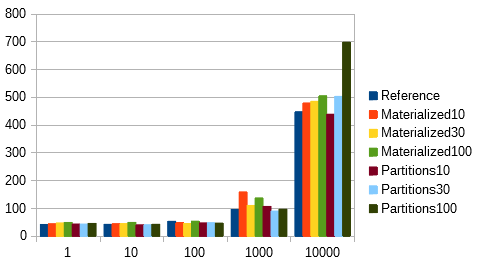
\includegraphics[scale=0.8]{charts/Query1.png}
    \caption{Average query execution time in milliseconds of $Q_1$ (Appendix~\ref{app:queries})}
    \label{fig:query1}
\end{figure}

For the second query, $Q_2$, the reference implementation's average query execution time took with increasing relation sizes always longer than any
implementation of the developed approaches (cf. Figure~\ref{fig:query2}). Even for the smaller scaling factors except for the SF of 1, the execution time was
slightly longer and for the highest scaling factor the execution time of almost five seconds was approximately 50 times as long as the other execution times.
This is because the reference implementation is unlike the developed approaches not capable of answering queries similarity-based as it lacks the
clustering-based fragmentation for the relaxation attribute. The developed approaches, on the contrary, are able to perform similarity-based query answering 
(cf. Section~\ref{sec:meth_sbqa}) for this query as it contains a selection condition on the relaxation attribute. Thus after identification of the relevant
fragment and query rewriting, the query execution is optimized.

\begin{figure}[h]
    \centering
    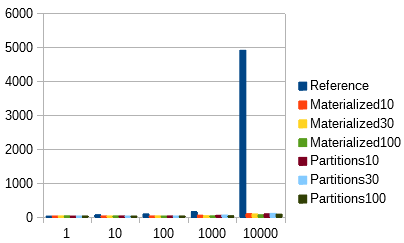
\includegraphics[scale=0.9]{charts/Query2.png}
    \caption{Average query execution time of $Q_2$ (Appendix~\ref{app:queries})}
    \label{fig:query2}
\end{figure}

To demonstrate the small differences in the query execution time for the other approaches, the next chart (Figure~\ref{fig:query2withoutref}) plots the same
execution times without the measurements of the reference implementation that are beyond the scope. Two interesting things illustrated in this chart are that,
firstly, both approaches approximately coincide with the execution times and, secondly, both approaches have their fastest execution times (SF=1000 and
SF=10000) for the whole term set compared to the other term set sizes. This is due to the fact that if there are less terms underlying the clustering, then 
more patients will have a tuple in the \verb!ILL! relation with the disease term \verb!'Liver Failure'! as the data is generated completely randomly and
diseases are picked randomly from the chosen term set. This results in more tuples matching the selection condition and also more tuples that have to be joined,
whereas the join is still pretty fast due to collocation, but a presumably bigger result set has to be transferred back to the client.

\begin{figure}[h]
    \centering
    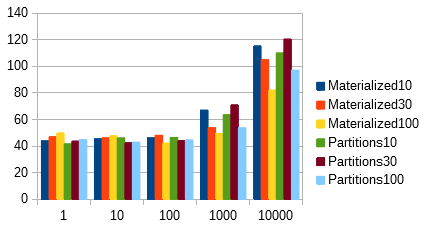
\includegraphics[scale=0.9]{charts/Query2WithoutReference.png}
    \caption{Average query execution time of $Q_2$ (Appendix~\ref{app:queries}) without reference implementation}
    \label{fig:query2withoutref}
\end{figure}


The situation for query 3 from Appendix~\ref{app:queries} is almost the same as for query 2 because as depicted in Figure~\ref{fig:query3} the average execution
time of the query was multiple times higher for the reference implementation, too. Here, the measurement was even approximately 600 times higher for the biggest
database size (SF=10000). In comparison to the previous query, this behaviour can be explained by the fact that the relation \verb!ILL! is joined with itself in
the query's \verb!FROM! clause instead of only once with the \verb!INFO! relation. In case of the distributed data, this query answer calculation is 
computationally expensive. One possible execution for the DDBS is to separately collect all tuples from the \verb!ILL! relation that either satisfy the first 
selection condition (\verb!i1.disease = 'Liver Failure'!) or the second one (\verb!i1.disease = 'Hemoptysis'!) on one server in two sets that are joined after 
the collection via the shared attribute (\verb!i1.id = i2.id!). This join is not explicitly formulated in the query but it can be concluded implicitly from the 
transitivity of the "\verb!=!-chain" in the \verb!WHERE! clause. In the last step, the joined tuples have to be joined again with the \verb!INFO! relation that 
is distributed and requires for transferring tuples between the servers. A more efficient execution is achieved by pushing down the join with the \verb!INFO!
tuples as the collocation allows for a local join and avoids costly data transfer.
\begin{figure}[h]
    \centering
    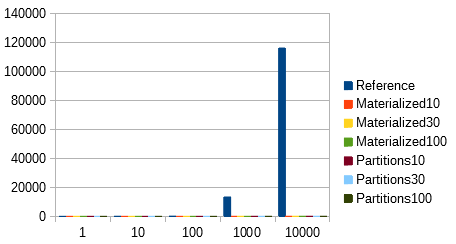
\includegraphics[scale=0.9]{charts/Query3.png}
    \caption{Average query execution time of $Q_3$ (Appendix~\ref{app:queries})}
    \label{fig:query3}
\end{figure}


Figure~\ref{fig:query3withoutref} depicts the same time measurements as before without the execution times of the reference implementation which are again beyond
the scope. Here, one can see that the average execution time of $Q_3$ has an equal length for the three smallest scaling factors and only increases for the
biggest two factors. The main reason for this behaviour is first of all the increased amount of data. But as the comparison to Figure~\ref{fig:query2withoutref}
reveals, the query execution of $Q_3$ takes around 100ms longer (SF=10000) than the execution of $Q_2$. This is due to the fact that the similarity-based query
answering technique (cf. Section~\ref{sec:meth_sbqa}) identifies two fragments, one corresponding to the cluster where the disease term "Liver Failure" belongs
to and one corresponding to the cluster where the disease term "Hemoptysis" belongs to, where, in contrast to this, for answering $Q_2$ the former suffices. 
Furthermore, the tuples of those two fragments need to be joined in order to provide the correct result set which can be performed locally in the optimal case,
i.e. when both fragments are hosted by the same server, but involves data transfer between the two servers if the fragments do not reside at the same server.
Due to this reasons, the execution of $Q_3$ is slightly slower than $Q_2$ but still the developed approaches outperform the reference implementation.
\begin{figure}[h]
    \centering
    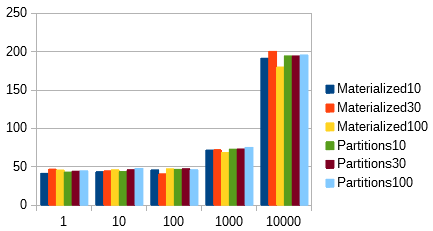
\includegraphics[scale=0.9]{charts/Query3WithoutReference.png}
    \caption{Average query execution time of $Q_3$ (Appendix~\ref{app:queries}) without reference implementation}
    \label{fig:query3withoutref}
\end{figure}


The average execution times for $Q_4$ (Figure~\ref{fig:query4}) and $Q_5$ (Figure~\ref{fig:query5}) show again only few differences between all 
implementations for the smaller database sizes. But as the size is increased by a factor of 10000, both queries are executed approximately 5 to 7 times as long 
in the materialized fragment approach than compared to the reference implementation whereas the other approach is only slightly slower (up to twice as long).
Because of the requirement to rewrite the queries in the materialized fragment approach according to the localization program of the underlying fragmentation,
the average execution time takes significantly longer in this approach as the rewritten query comprises one subquery per fragment that are all connected in a 
big SQL \verb!UNION!, e.g. for $n$ fragments the rewritten query $Q_{rewritten}$ is
\begin{verbatim}
    (SELECT ... FROM ILL_0 i, INFO_0 p WHERE ...)
    UNION
    (SELECT ... FROM ILL_1 i, INFO_1 p WHERE ...)
    UNION
    ...
    UNION
    (SELECT ... FROM ILL_n i, INFO_n p WHERE ...)
\end{verbatim}
(cf. Example~\ref{sec:theo_dqp_exmp2}). The stair-like appearance of the three corresponding bars (orange, yellow, green) mirror the total number of clusters 
and fragments of the relations from the underlying clustering-based fragmentation This complex and long query can not be executed as fast as the non-rewritten
queries. A reason why the query execution in the partition number approach is a little bit slower than the reference implementation could be a disadvantageous
distribution of data to the different fragments leading to a non-optimal performance when executing the query. Additionally, the by \citetalias{Ignite} provided
automatic partitioning and distribution of the data can be handled in a more balanced way as the DDBS strives to equalize the load on all participating nodes
yielding a more balanced data distribution that might be more advantageous for execution of the queries in comparison to the clustering-influenced distribution
of the developed approaches.
\begin{figure}[h]
    \centering
    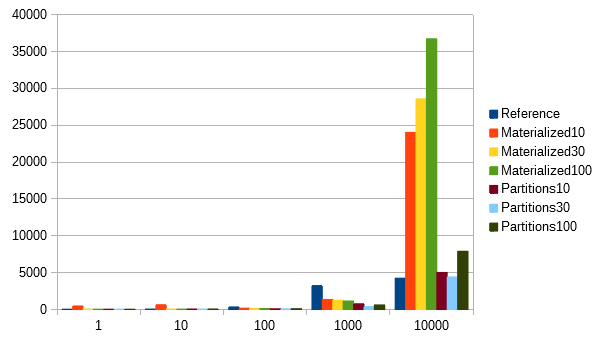
\includegraphics[scale=0.8]{charts/Query4.png}
    \caption{Average query execution time of $Q_4$ (Appendix~\ref{app:queries})}
    \label{fig:query4}
\end{figure}

\begin{figure}[h]
    \centering
    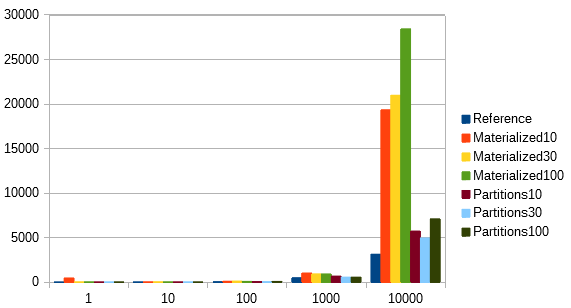
\includegraphics[scale=0.8]{charts/Query5.png}
    \caption{Average query execution time of $Q_5$ (Appendix~\ref{app:queries})}
    \label{fig:query5}
\end{figure}



The time measurements for the execution of $Q_6$ are illustrated in Figure~\ref{fig:query6}. The execution of this query was only investigated for the scaling 
factors 1, 10 and 100 as for the bigger factors the query execution time exceeded the timeout threshold of 10 minutes. The interesting points here are firstly
coincidence of the measurements for the reference implementation with the measurements of the partition number approach and secondly the stair-like shape of
the bars that belong to execution times of the materialized fragment approach as already seen before for $Q_4$ and $Q_5$. The higher execution times for the
materialized fragment approach are caused by the complexity of the rewritten query that looks very similar to the previously sketched $Q_{rewritten}$ but as the
initial query contains a join of the relation \verb!ILL! with itself the corresponding localization program has to consider all pairs of two materialized
\verb!ILL! fragments, i.e. for each materialized fragment table there is a subquery that has the same structure as $Q_{rewritten}$ with an additional join of
that certain fragment table and all the subqueries, which are unions of subqueries themselves, are aggregated by \verb!UNION!s to one final query. The impact of
this nesting of subqueries connected by unions on the query execution performance increases exponentially with the number of joined relations.

\begin{figure}[h]
    \centering
    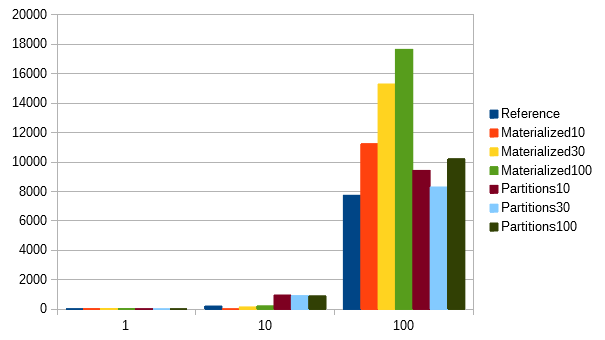
\includegraphics[scale=0.8]{charts/Query6.png}
    \caption{Average query execution time of $Q_6$ (Appendix~\ref{app:queries})}
    \label{fig:query6}
\end{figure}


\todo[inline]{FAQ}

% Appendix
\newpage
\appendix
%!TEX root = jsba_main.tex

% Appendix
\section{Appendix}


% Bibliography
\newpage
\bibliography{literature}

\end{document}
